\documentclass[aps,prl,reprint]{revtex4-1}
\usepackage{blindtext}

\usepackage{amsmath}
\usepackage{graphicx}
\usepackage{commath}
\usepackage{siunitx}
\usepackage{tabularx}
\usepackage{subcaption}

\usepackage{amssymb}

\usepackage{float}

\usepackage{graphicx}


\usepackage[b]{esvect}


\newcommand{\de}{\mathrm{d}}
\newcommand{\vcc}{V_\text{CC}}
\newcommand{\parallelsum}{\mathbin{\!/\mkern-5mu/\!}}


\graphicspath{ {images/} }
\begin{document}

\title{Unit 5: Negative Feedback and Operational Amplifiers}
\author{Xueqi Li}
% \email{xueqi.li@stonybrook.edu}
\thanks{Partner: Tianming Hai}
% \author{partner Tianming Hai}
\noaffiliation
\date{Apr 14, 2018}


% \begin{abstract}
% Here I tell what I have done... And I have done a lot but it is hard to tell what exactly I have done...
% \end{abstract}

\maketitle

\section{Introduction}  
    An operational amplifier (opamp) can amplifie the input voltage by a large factor. Since it have a large gain, it might not stable in many case and the output is very uncontrollable, we usualy build up a circuits with it to achieve a much stable circuit.

    An opamp, other than power-supply pins ($\vcc$ and $V_\text{EE}$), have two input and one output, where the input are known as non-inverting input (+) and inverting input ($-$). The ouput is given as:
    \begin{equation}
        v_\text{out} = A_0 (v_+ - v_-) \label{eq:opamp}
    \end{equation}

where $A_0$ is a very large number. Usually it is higher than $10^5$. The impedance of the opamp can be think as ideal.
    \subsection{Negative Feedback}
        A negative feedback is such that the output of the opamp connect to the inverting input. That is to say, $v_- = v_\text{out}$. This leads to following equation:
        \begin{subequations}
            \begin{align}
                v_+ &= v_- \label{eq:veq}  \\
                i_+ &= i_- = 0 \label{eq:ieq}
            \end{align}
        \end{subequations}

    \subsection{Follower}
        \begin{figure}[h]
            \centering
            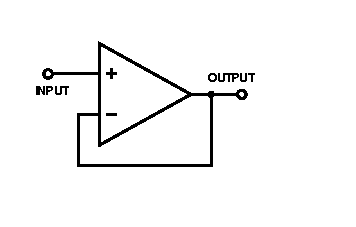
\includegraphics[height=1in]{image/Amp-Follower.pdf}
            \caption{A follower}
            \label{fig:follower}
        \end{figure}{}
        The simplest negative feedback circuit is a follower, so as in Figure~\ref{fig:follower}. From Equation~\ref{eq:veq}, we see that
        \begin{equation}
            V_\text{out} = V_\text{in}
        \end{equation}
    \subsection{Inverting Amplifier}
        \begin{figure}[h]
            \centering
            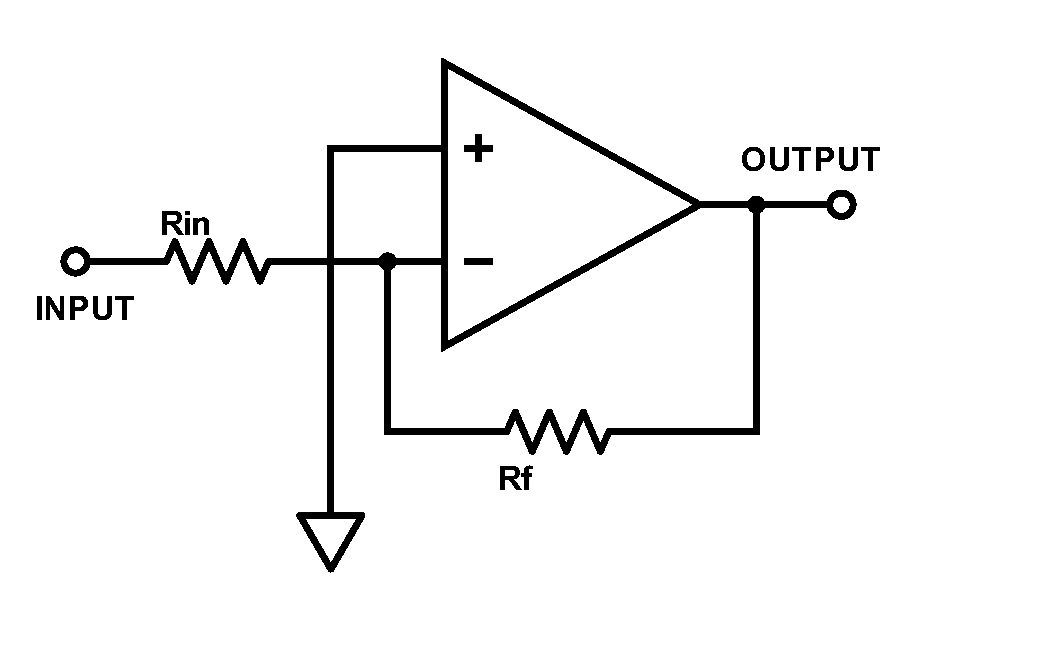
\includegraphics[height=1in]{image/Inverting-Amp.pdf}
            \caption{An Inverting Amplifier}
            \label{fig:invertingAmplifier}
        \end{figure}{}
        An operational amplifier have to be able to be an amplifier! An Inverting Amplifier is presented as Figure~\ref{fig:invertingAmplifier}. Since the non-inverting input is grounded, we must have $v_+ = v_- = 0$V. Thus, we can find the current in the input side are given as
        \[
        I_\text{in} = \frac{V_\text{in}}{R_\text{in}}
        \]
        Follow the Equation~\ref{eq:ieq}, this current have to be also go through $R_f$, where the voltage drop on $R_f$ just so happened to be output voltage ($v_- - V_\text{out}$):
        \begin{align}
            V_\text{out} = - I R_f = - V_\text{in}\frac{R_f}{R_\text{in}} \label{eq:invertingAmplifier}
        \end{align}
        where we see that the gain is just given as:
        \[
            \text{Gain} = - \frac{R_f}{R_\text{in}}
        \]
        Notice that for the inverting amplifier, the input impedance is give as:
        \begin{align*}
            Z_\text{in} = \frac{\de V_\text{in}}{\de I_\text{in}} = R_\text{in}
        \end{align*}
        which is not a very high input impedance. In the other hand, easy to see the output impedance is ideal.

    \subsection{Non-inverting Amplifier}
        \begin{figure}[h]
            \centering
            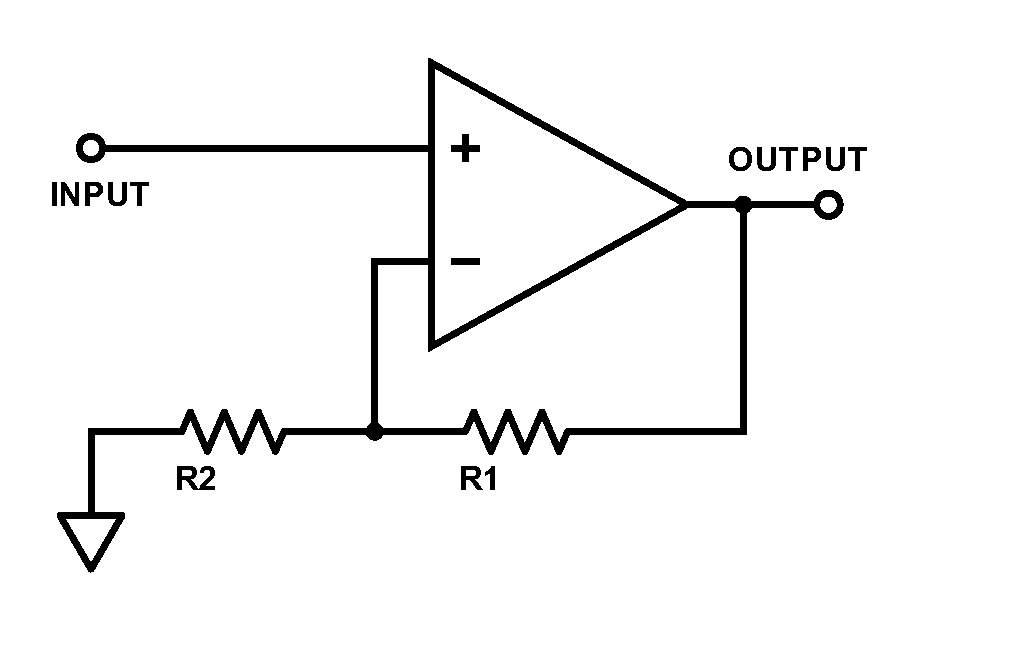
\includegraphics[height=1in]{image/Non-inverting-Amp.pdf}
            \caption{An non-inverting Amplifier}
            \label{fig:nonInvertingAmplifier}
        \end{figure}{}
        It is nice to have a non-inverting amplifier. A non-inverting amplifier is shown as Figure~\ref{fig:nonInvertingAmplifier}. Since the input is directly connect to the non-inverting input, we have $V_\text{input} = v_+ = v_-$. In the end of $R_2$, we must have 0V sicne it is grounded. Thuse we have:
        \[
            I_2 = \frac{V_\text{in}}{R_2}
        \]
        From Equation~\ref{eq:ieq}, this current have to go through $R_1$:
        \[
            V_1 = I R_1 = V_\text{in} \frac{R_1}{R_2}
        \]
        where the other end of $R_2$ just so happened to be the output:
        \begin{equation}
            V_\text{output} = V_\text{in} + V_1 =  V_\text{in} (1+ \frac{R_1}{R_2}) \label{eq:nonInvertingAmplifier}
        \end{equation}
        which give as a gain as:
        \[
            \text{Gain} = (1+ \frac{R_1}{R_2})
        \]

    \subsection{Integrator}
        \begin{figure}[h]
            \centering
            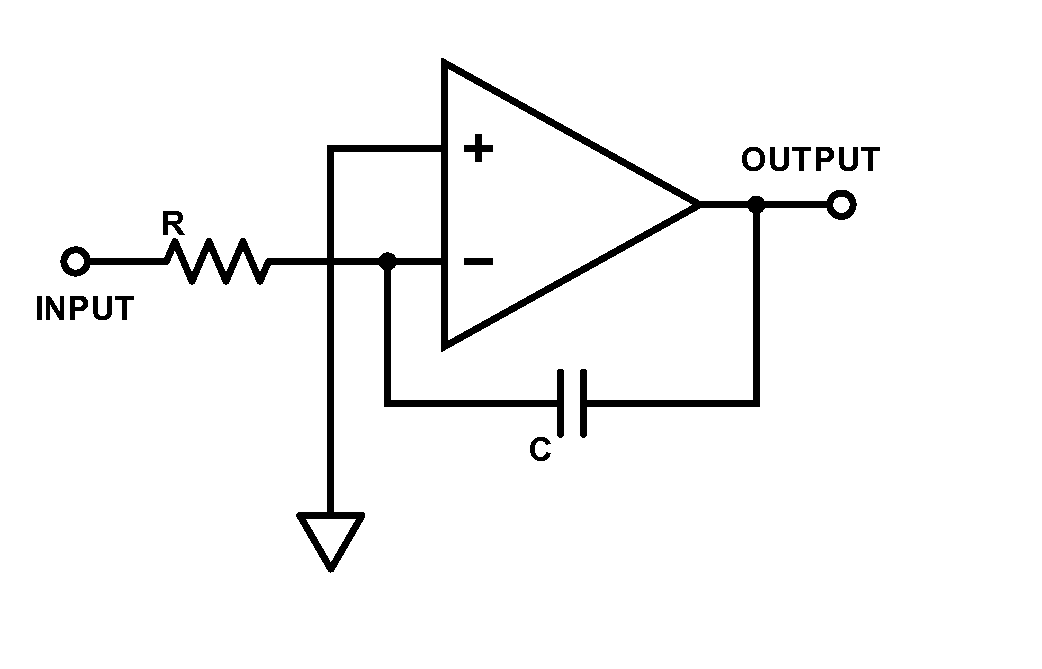
\includegraphics[height=1in]{image/Integrator.pdf}
            \caption{An Integrator}
            \label{fig:integrator}
        \end{figure}{}
        The circuit presented in Figure~\ref{fig:integrator} is an integrator. Since the non-inverting input is grounded, we have $v_- = v_+ = 0$V. Thus we can find the current in the capacitor is the same as the current go through the resistor:
        \[
        I = -C \frac{\de V_\text{out}}{\de t} = \frac{V_\text{in}}{R}
        \]
        solve the equation, we have:
        \begin{equation}
            V_\text{out} = - \frac{1}{RC} \int V_\text{in} \de t \label{eq:integrator}
        \end{equation}

        However, there is a problem for the integrator. Usually, the input might have an offset. That is to say, there is a constent term in the input voltage. This will give us a growing or falling output after integration. To solve it, one can parallel a resistor with the capacitor.
        \subsubsection{T Network}
            \begin{figure}[h]
                \centering
                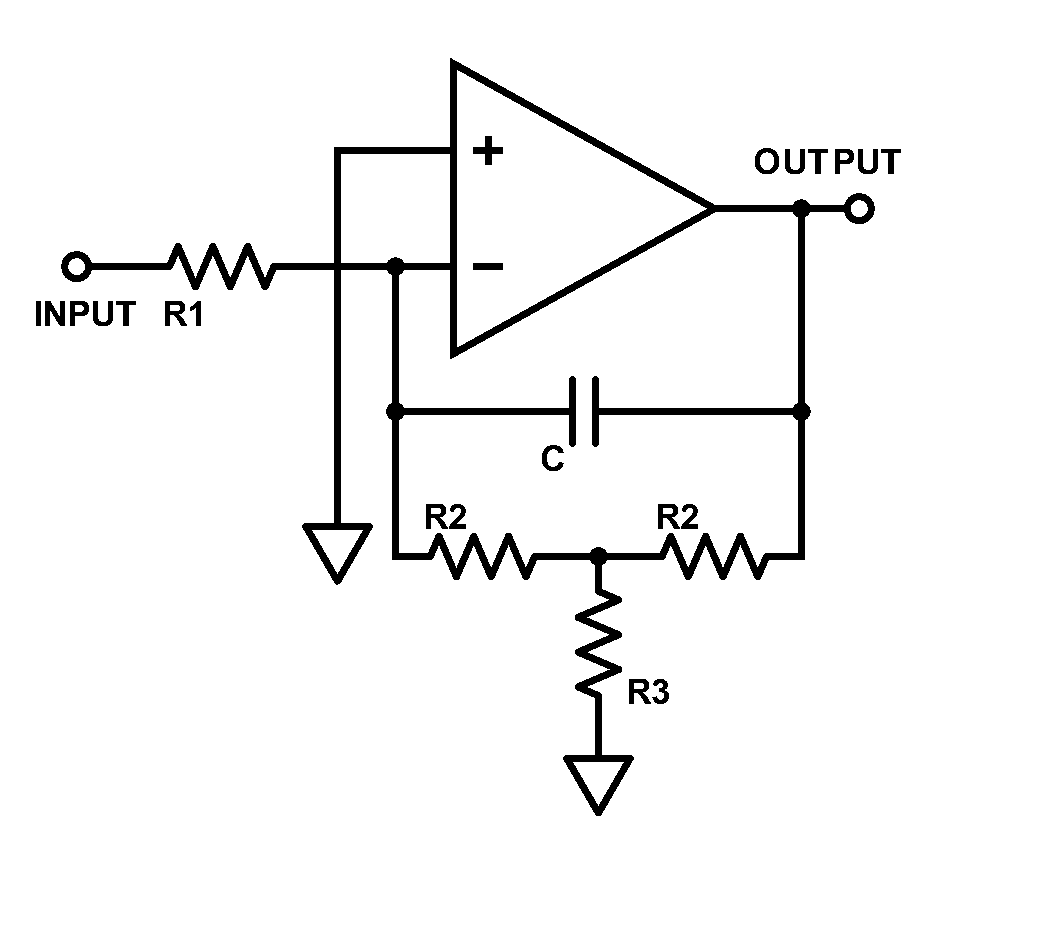
\includegraphics[height=1.3in]{image/T-network.pdf}
                \caption{An Integrator with T network}
                \label{fig:tNetwork}
            \end{figure}{}
            To achieve a large parallel resistor, one can use a T network, so as in Figure~\ref{fig:tNetwork}. Ignore the capacitor, we can just calculate the effect of the T network. First, we still have the current on the $R_1$ will go through the left $R_2$:
            \[
            I_1 = \frac{V_\text{in}}{R_1} = I_\text{2L} = I_\text{2R} + I_3
            \]
            On the other hand, the voltage between $R_1$ and $R_\text{2L}$ is 0V. Thus we can find the voltage between two $R_2$:
            \[
            V_2 = 0 - I_1 R_2 = - V_\text{in} \frac{R_2}{R_1}
            \]
            And this voltage will dorp to zero once it go through $R_3$:
            \[
            I_3 = \frac{V_2}{R_3} = - V_\text{in} \frac{R_2}{R_1 R_3}
            \]
            In the output end, we can write the current go through $R_2$ as following:
            \[
            I_2 = \frac{V_2 - V_\text{out}}{R_2} = -\frac{V_\text{in}}{R_1} - \frac{V_\text{out}}{R_2}
            \]
            This relate the output voltage to the current. Now we have $I_1 = I_2 + I_3$:
            \[
            \frac{V_\text{in}}{R_1} =  - V_\text{in} \frac{R_2}{R_1 R_3} -\frac{V_\text{in}}{R_1} - \frac{V_\text{out}}{R_2}
            \]
            Solve the equation, we find
            \[
            V_\text{out} = - V_\text{in} \frac{R_2}{R_1} (2 + \frac{R_2}{R_3})
            \]
            This give us the impedance of the T network:
            \[
            Z_f = R_2(2 + \frac{R_2}{R_3})
            \]
            Thus, we can achieve a high impedance if we just chose two two small resistor with a large ratio.
    \subsection{Differentiator}
        \begin{figure}[h]
            \centering
            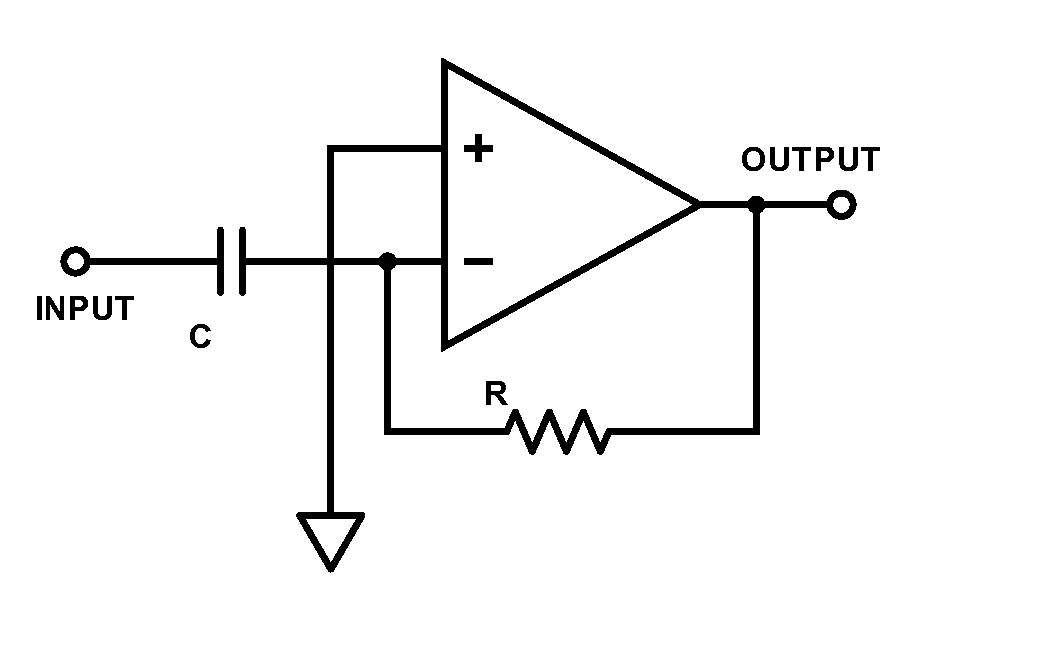
\includegraphics[height=1in]{image/Differentiator.pdf}
            \caption{An Differentiator}
            \label{fig:differentiator}
        \end{figure}{}
        By interchange the resistor and capacitor of integrator, one can achieve a differentiator, as in Figure~\ref{fig:differentiator}. Since the non-inverting input is grounded, we have to have 0V on $v_-$. This means the current go through the capacitor and the resistor are the same:
        \begin{equation}
            V_\text{out} = - IR = -RC \frac{\de V\text{in}}{\de t}
        \end{equation}

    \subsection{Limit of the Opamp}
        A realistic opamp are not ideal. There are a few importent things we have to consider when use it:
        \begin{enumerate}
            \item The voltage gain ($A_0$) will drop linearly to the frequency in logarithm scale;
            \item There might be a phase shift in the output;
            \item For the feedback loop, Equation~\ref{eq:ieq} is approximate, i.e., $i_+$, $i_- \approx 0$;
            \item For the feedback loop, Equation~\ref{eq:veq} is approximate, i.e., $v_+ \approx v_-$;
            \item There is a small delay to the output. When input voltage change suddenly, the output voltage will learly increase and reach the theoretical value. This is called slew rate.
        \end{enumerate}
\section{Data and Calculation}


\section{Analysis}

\section{Conclusion}



\bibliography{cite}
\bibliographystyle{apsrev4-1}

    % \begin{figure}[h]
    %     \centering
    %     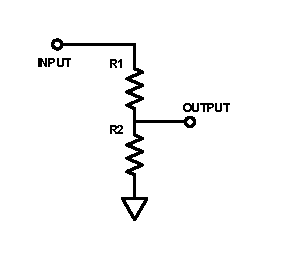
\includegraphics{images/plot2.pdf}
    %     \caption{A voltage divider}
    %     \label{fig:2}
    % \end{figure}

    % \begin{table}[h]
    % \begin{ruledtabular}
    % \begin{tabular}{cccc} 
    % Load[k$\Omega$] &  Output Voltage[V] & $R_\text{th}[\Omega]$ & Theoretical Voltage\\ \hline\hline
    % 50              & 0.680(1)           & 501(1)                & 0.682 \\ \hline
    % 500             & 3.75(1)            & 500(1)                & 3.75 \\ \hline
    % 5000            & 6.80(1)            & 514(1)                & 6.82 \\
    % \end{tabular}
    % \end{ruledtabular}
    % \caption{Load resistor and the output}
    % \label{table:8}
    % \end{table} 

% \begin{center}
%  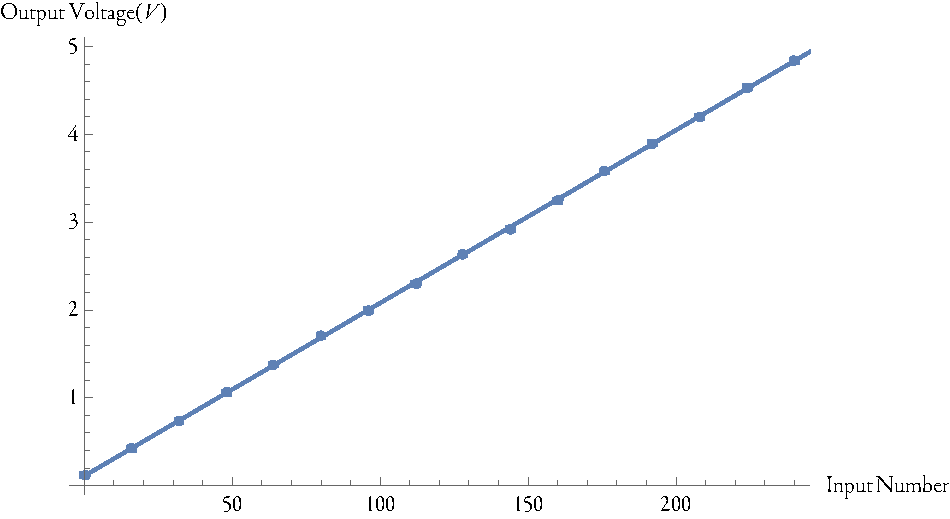
\includegraphics[height=1.8in]{plot.pdf}
% \end{center} 

%\begin{center}
% 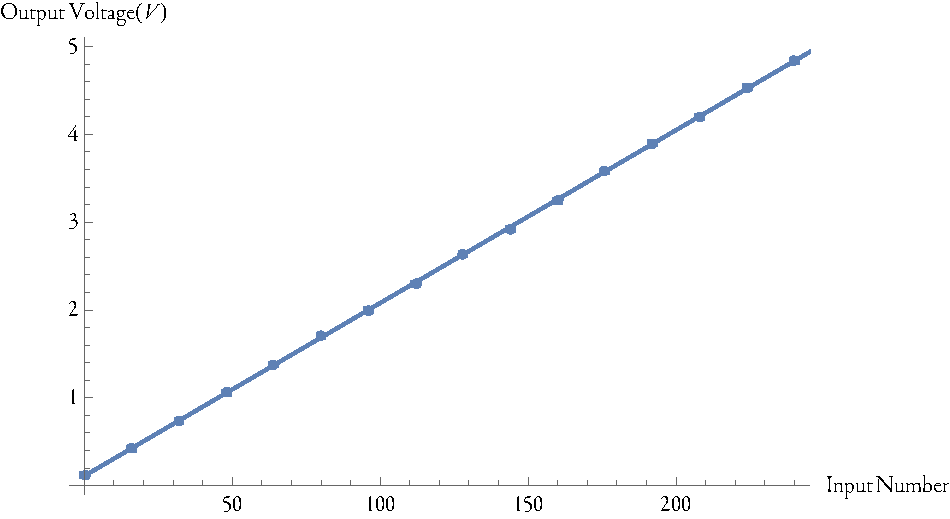
\includegraphics[height=1.3in]{plot.pdf}
%\end{center}

% \blindtext \cite{article-minimal}

% \bibliographystyle{apsrev4-1} % Tell bibtex which bibliography style to use
% \bibliography{xampl} % Tell bibtex which .bib file to use (this one is some example file in TexLive's file tree)

\end{document}